\section{神经网络}
\subsection{神经网络的基本概念}
神经网络包含一个输入层,若干个隐藏层和一个输出层。每一层的每一个神经元都会经过\textbf{激活函数}从而输出一个值,
常见的激活函数包括 Sigmoid 函数、ReLU 函数等。

下面对神经网络中一些记号进行解释:
\begin{itemize}
    \item $a_i^{(j)}$ 表示第 $j$ 层第 $i$ 个神经元或单元的激活项,激活项是指由一个具体的神经元计算并输出的值;
    \item $\Theta^{(j)}$ 表示控制从第 $j$ 层到第 $j+1$ 层的映射的权重矩阵。
\end{itemize}

如果第 $j$ 层有 $s_j$ 个单元,$j+1$ 层有 $s_{j+1}$ 个单元,
则 $\Theta^{(j)}$ 的维数为 $s_{j+1} \times (s_j + 1)$。

\subsection{神经网络的前向传播}
在神经网络中,信息从上一个神经元直接流转到下一个神经元,
直到输出,依据每一个神经元的输入并根据相应规则可以计算出输出,最终得到在当前参数下的损失函数的过程,称为\textbf{前向传播}。其计算公式为:
\begin{equation}
    \begin{cases}z^{(i+1)} = \Theta^{(i)}a^{(i)} \\ a^{(i+1)} = g\left(z^{(i+1)}\right)\end{cases}
\end{equation}
    
其中 $g(x)$ 为激活函数,$a^{(i)}$ 为第 $i$ 层的激活项,$z^{(i+1)}$ 为第 $i+1$ 层的输入项。

\begin{example}
    构造一个神经网络用以计算 $x_1 \operatorname{XNOR} x_2$。

    考虑逻辑推导同或,由于 $A \bigoplus B = \overline A B + A \overline B$,由德摩根律得 
    $A \operatorname{XNOR} B = \overline{\left(\overline A B + A \overline B\right)} = \overline{AB} + AB$。

    根据此,我们可以构造一个神经网络:
    
   \begin{center}
    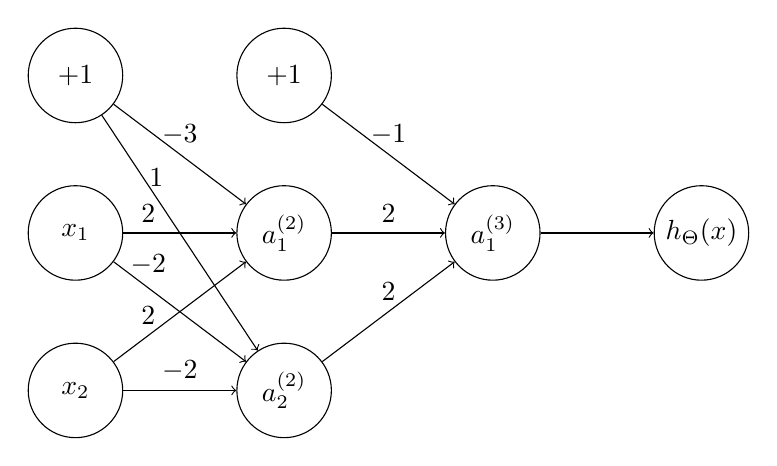
\begin{tikzpicture}[
    neuron/.style={circle,draw,inner sep=0pt,minimum size=12mm}
    ]
    
    \node (a12) at (0, 0) [neuron] {$a_1^{(2)}$};
    \node (a02) at (0, 2) [neuron] {$+1$};
    \node (a22) at (0, -2) [neuron] {$a_2^{(2)}$};
    \node (x0) at (-2.65, 2) [neuron] {$+1$};
    \node (x1) at (-2.65, 0) [neuron] {$x_1$};
    \node (x2) at (-2.65, -2) [neuron] {$x_2$};
    \node (a13) at (2.65, 0) [neuron] {$a_1^{(3)}$};
    \node (output) at (5.3, 0) [neuron] {$h_\Theta(x)$};
    \draw [->] (x0) to node [yshift=2.5mm] {$-3$} (a12);
    \draw [->] (x0) to node [xshift=-3mm, yshift=7mm] {$1$} (a22);
    \draw [->] (x1) to node [xshift=-4mm, yshift=2.5mm] {$2$} (a12);
    \draw [->] (x1) to node [xshift=-4mm, yshift=6mm] {$-2$} (a22);
    \draw [->] (x2) to node [xshift=-4mm, yshift=-0.5mm] {$2$} (a12);
    \draw [->] (x2) to node [yshift=2.5mm] {$-2$} (a22);
    \draw [->] (a02) to node [yshift=2.5mm] {$-1$} (a13);
    \draw [->] (a12) to node [yshift=2.5mm] {$2$} (a13);
    \draw [->] (a22) to node [yshift=2.5mm] {$2$} (a13);
    \draw [->] (a13) to (output);
  \end{tikzpicture}
   \end{center} 

  通过简单的计算我们得到,$a_1^{(2)}$ 计算得到的结果是 $AB$,
  $a_2^{(2)}$ 计算得到的结果是 $\overline{AB}$,$a_1^{(3)}$ 计算得到的结果是 $\overline{AB} + AB$,是我们需要的结果。
\end{example}

\subsection{神经网络解决多分类问题}
在神经网络中,我们可以通过将输出层的神经元个数设置为类别的个数,从而解决多分类问题。
例如,我们有三个类别,那么我们可以将输出层的神经元个数设置为 $3$,
并且将每个神经元的激活函数设置为 Sigmoid 函数,从而得到每个类别的概率。

之后,我们对所有输出层的输出值求 $\max$,得到最大的概率对应的类别即为预测结果。

\subsection{神经网络的代价函数}
在神经网络中,我们使用交叉熵作为代价函数:
假设 $h_\Theta(x) \in \mathbb{R}^K$,
$\left(h_\Theta(x)\right)_i$ 表示神经网络中输出向量的第 $i$ 个输出,即向量中的第 $i$ 项,则代价函数表示为
\begin{equation}
    \begin{aligned}
        J(\Theta) = &-\dfrac 1m\left[\sum\limits_{i=1}^m{\sum\limits_{k=1}^K{y_k^{(i)}\log (h_\Theta(x^{(i)})_k) + (1 - y_k^{(i)}) \log (1 - (h_\Theta(x^{(i)}))_k)}}\right] \\ 
        &+ \dfrac \lambda{2m}\sum\limits_{l=1}^{L-1}{\sum\limits_{i=1}^{s_l}{\sum\limits_{j=1}^{s_{l+1}}\left(\Theta_{ji}^{(l)}\right)^2}}
    \end{aligned}
\end{equation}

\begin{proof}
对于此函数,直观的理解是将其与逻辑回归的代价函数做对比,由于神经网络中输出是一个 $\mathbb{R}^K$ 的向量,
于是必须存在一个求和将这些输出单元的代价加起来,这就有了内层的求和号;

对于第 $k$ 个输出单元,它预测的类别是 $h_\Theta(x^{(i)})_k$,实际的类别是 $(y^{(i)})_k$,
将其在逻辑回归的代价函数中做替换即可得到神经网络代价函数中的前一项;

而后一项明显为 L2 正则项,逻辑回归中是将除 $\theta_0$ 以外的所有参数平方后求和,
类比到神经网络中,以 $a_1^{(i+1)}$ 举例,它会和 $a_1^{(i)}, a_2^{i}, \dots, a_{s_{i}}^{(i)}$ 这 $s_{i}$ 个神经元相连,
相连时的参数分别为 $\Theta_{11}^{(i)}, \Theta_{12}^{(i)}, \dots, \Theta_{1s_i}^{(i)}$,那么这个神经元表示的逻辑回归即为
\begin{equation}
    a_1^{(i+1)} = \sum\limits_{j=0}^{s_i}{\Theta_{1j}^{(i)}a_j^{(i)}}
\end{equation}
那么这一个逻辑回归对应的 L2 正则项为
\begin{equation}
    \sum\limits_{j=1}^{s_i}\left({\Theta_{1j}^{(i)}}\right)^2
\end{equation}
将第 $i+1$ 层的 $s_{i+1}$ 个神经元都考虑进来得到
\begin{equation}
    \sum\limits_{j=1}^{s_i}{\sum\limits_{k=1}^{s_{i+1}}\left({\Theta_{kj}^{(i)}}\right)^2}
\end{equation}
再把第 $1$ 层到第 $L-1$ 层考虑进来便得到神经网络代价函数中的后一项。
\end{proof}

\subsection{反向传播算法}
反向传播算法是一个让代价函数最小化的算法。
为了使用梯度下降法来找到 $\underset{\Theta}{\arg \min}\ J(\Theta)$,
我们需要计算 $J(\Theta)$ 和 $\dfrac{\partial}{\partial \Theta_{ij}^{(l)}}J(\Theta)$ 的值,从而能够使用梯度下降。

\subsubsection{每层只有一个神经元的情况}

考虑最后一层的激活值是如何计算的:
\begin{equation}
    a^{(L)} = g\left(\omega^{(L)}a^{(L-1)} + b^{(L)}\right) = g\left(z^{(L)}\right)
\end{equation}

这个过程如下图所示:
\begin{center}
    \begin{tikzpicture}[
        neuron/.style={circle,draw,inner sep=0pt,minimum size=12mm}
        ]
    
        \node (aL-1) at (0, 0) [neuron] {$a^{(L-1)}$};
        \node (wL) at (-2.65, 0) [neuron] {$\omega^{(L)}$};
        \node (bL) at (2.65, 0) [neuron] {$b^{(L)}$};
        \node (zL) at (0, -2.65) [neuron] {$z^{(L)}$};
        \node (aL) at (0, -5.3) [neuron] {$a^{(L)}$};
        \node (y) at (-2.65, -5.3) [neuron] {$y$};
        \node (C0) at (0, -7.95) [neuron] {$C_0$};
        \draw (wL) to (zL);
        \draw (aL-1) to (zL);
        \draw (bL) to (zL);
        \draw (zL) to (aL);
        \draw (y) to (C0);
        \draw (aL) to (C0);
      \end{tikzpicture}
\end{center}

下面假设代价函数为均方误差。考虑计算当 $\omega^{(L)}$ 变化时,代价函数的变化程度,即
\begin{equation}
    \dfrac{\partial}{\partial \omega^{(L)}} C_0
\end{equation}
根据求导的链式法则有
\begin{equation}
    \dfrac{\partial}{\partial \omega^{(L)}} C_0 = \dfrac{\partial z^{(L)}}{\partial \omega^{(L)}} 
    \cdot \dfrac{\partial a^{(L)}}{\partial z^{(L)}} \cdot \dfrac{\partial C_0}{\partial a^{(L)}}
\end{equation}
下面计算右侧各式的值:
\begin{equation}
    \begin{aligned}
        \dfrac{\partial C_0}{\partial a^{(L)}} &= \dfrac{\partial }{\partial a^{(L)}} \dfrac 12 \left(a^{(L)} - y\right)^2= \left(a^{(L)} - y\right) \\
        \\
        \dfrac{\partial a^{(L)}}{\partial z^{(L)}} &= \dfrac{\partial}{\partial z^{(L)}} g\left(z^{(L)}\right)= \dfrac{\partial}{\partial z^{(L)}} z^{(L)} \cdot g'\left(z^{(L)}\right) = g'\left(z^{(L)}\right) \\
        \\
        \dfrac{\partial z^{(L)}}{\partial \omega^{(L)}} &= \dfrac{\partial}{\partial \omega^{(L)}} \left(\omega^{(L)}a^{(L-1)} + b^{(L)}\right) = a^{(L-1)}
        \end{aligned}
\end{equation}

\subsubsection{每层有多个神经元的情况}
我们令 $j$ 表示最后一层的第 $j$ 个神经元,$k$ 表示倒数第二层的第 $k$ 个神经元,此时最后一层的代价为
\begin{equation}
    C_0 = \dfrac 12 \sum\limits_{j=0}^{s_L-1}{\left(a_j^{(L)} - y_j\right)^2}
\end{equation}
再次提醒,$\omega^{(L)}_{jk}$ 表示 $L - 1$ 层的第 $k$ 个神经元连向 $L$ 层的第 $j$ 个神经元的权重,与单神经元类似地,令
\begin{equation}
    z_j^{(L)} = \sum\limits_{k=0}^{s_{L-1}-1} {\omega_{jk}^{(L)}a_k^{(L-1)}} + b_j^{(L)}
\end{equation}
则最后一层的激活值为
\begin{equation}
    a_j^{(L)} = g\left(z_j^{(L)}\right)
\end{equation}
其中 $g(x)$ 为 Sigmoid 函数。再次利用求导的链式法则,我们得到
\begin{equation}
    \begin{aligned}
        \dfrac{\partial C_0}{\partial \omega^{(L)}} &= \sum\limits_{k=0}^{s_{L-1}-1}a_k^{(L-1)}g'\left(z^{(L)}\right)\left(a^{(L)} - y\right) \\
        \\
        \dfrac{\partial C_0}{\partial b^{(L)}} &= 1g'\left(z^{(L)}\right)\left(a^{(L)} - y\right) \\
        \\
        \dfrac{\partial C_0}{\partial a_k^{(L-1)}} &= \sum\limits_{j=0}^{s_L-1}\omega_{jk}^{(L)}g'\left(z^{(L)}\right)\left(a^{(L)} - y\right)
        \end{aligned}
\end{equation}

\subsubsection{梯度下降的具体过程}
\begin{itemize}
    \item 先进行一次前向传播
    \begin{equation}
        \begin{cases}
            z^{(l)} = \omega^{(l)}a^{(l-1)} + b^{(l)} \\
            a^{(l)} = g\left(z^{(l)}\right)
            \end{cases}
    \end{equation}
    \item 计算输出层误差方程,按定义有
    \begin{equation}
        \delta_j^{(L)} = \dfrac{\partial C}{\partial z_j^{(L)}}
    \end{equation}
    由求导的链式法则得到
    \begin{equation}
        \delta_j^{(L)} = \dfrac{\partial C}{\partial a_j^{(L)}} g'\left(z_j^{(L)}\right) \quad {(\text{BP}1)}
        \label{BP1} 
    \end{equation}
    写作矩阵形式为
    \begin{equation}
        \delta^{(L)} = \nabla_aC \odot g'\left(z^{(L)}\right)
    \end{equation}
    其中 $\odot$ 表示按元素的乘积,有时也被称为 Hadamard 乘积或 Schur 乘积。举例:
    \begin{equation*}
        \begin{bmatrix}1 \\ 2\end{bmatrix} \odot 
        \begin{bmatrix}3 \\ 4\end{bmatrix} = 
        \begin{bmatrix}1 * 3 \\ 2 * 4\end{bmatrix} = \begin{bmatrix}3 \\ 8\end{bmatrix}
    \end{equation*}
    \item 再通过下一层的误差 $\delta^{(l+1)}$ 表示当前层的误差 $\delta^{(l)}$
    \begin{equation}
        \delta^{(l)} = \left((\omega^{(l+1)})^\mathrm{T}\delta^{(l+1)}\right) \odot g'\left(z^{(l)}\right) \quad (\text{BP}2)
        \label{BP2}
    \end{equation}
    \item 通过梯度下降更新权重 $\omega$ 和偏置值 $b$
    \begin{equation}
        \begin{cases}
            \omega_{jk}^{(l)} := \omega_{jk}^{(l)} - a_k^{(l-1)}\delta_j^{(l)} \\
            \\
            b_j^{(l)} := b_j^{(l)} - \delta_j^{(l)}
        \end{cases}
    \end{equation}
\end{itemize}

\begin{proof}
   下面给出式 \ref{BP2} 的证明:
\begin{equation}
    \begin{aligned}
        \delta^{(l)} &= \dfrac{\partial C}{\partial z^{(l)}} \\
        \\
        &= \dfrac{\partial C}{\partial z^{(l+1)}} \cdot \dfrac{\partial z^{(l+1)}}{\partial a^{(l)}} \cdot \dfrac{\partial a^{(l)}}{\partial z^{(l)}} \\
        \\
        &= (\delta^{(l+1)} \cdot \omega^{(l+1)}) \odot g'\left(z^{(l)}\right)
    \end{aligned}
\end{equation}
由于 $\omega^{(l+1)}$ 维数为 $s_l \times s_{l+1}$,故上式也可以写作
\begin{equation}
    \delta^{(l)} = ((\omega^{l+1})^\mathrm{T}\delta^{(l+1)}) \odot g'\left(z^{(l)}\right)
\end{equation}
得证。 
\end{proof}

\subsection{梯度检查}

梯度检查是一个用来保证每次的前向传播、反向传播都是正确的算法。
当 $\theta \in \mathbb{R}^n$ 时,
此时 $\theta = \left[\theta_1, \theta_2, \dots, \theta_n\right]$,我们只需要对向量中每一个参数的偏导数都进行估计即可。具体地,
\begin{equation}
    \dfrac{\partial}{\partial \theta_i}J(\theta) = \lim\limits_{\epsilon \to 0} \dfrac{J(\dots, \theta_{i - 1}, \theta_i + \epsilon, \theta_{i+1}, \dots)
     - J(\dots, \theta_{i - 1}, \theta_i - \epsilon, \theta_{i+1}, \dots)}{2\epsilon}
\end{equation}

其中 $\epsilon$ 一般取 $10^{-4}$ 即可。

\textbf{在正式训练中不要使用梯度检查,因为计算代价相比于反向传播而言非常大。}

\subsection{随机初始化}
在神经网络中,对参数进行初始化时,我们需要使用随机初始化的思想。

具体地,令每个 $\Theta_{ij}^{(l)}$ 等于 $[-\epsilon, \epsilon]$ 内的一个随机数,即
\begin{equation}
    -\epsilon \leq \Theta_{ij}^{(l)} \leq \epsilon
\end{equation}

\subsection{总结}
\begin{itemize}
    \item 选择一个合适的神经网络架构:
    \begin{itemize}
        \item 输入层单元个数为特征向量的维度;
        \item 输出层单元个数为所要区分的类别个数。注意,每个数据的类别应当是一个\textbf{向量},而不是一个实数。
        \item 一般来说,默认只用一个隐藏层,如果使用多个隐藏层的话,默认每个隐藏层都具有相同数量的神经元。
    \end{itemize}
    \item 训练神经网络:
    \begin{itemize}
        \item 随机地初始化权重矩阵;
        \item 对于每个训练数据 $x^{(i)}$,执行前向传播以得到输出 $h_\Theta(x^{(i)})$;
        \item 计算代价函数 $J(\Theta)$;
        \item 执行反向传播计算所有的偏导数 $\dfrac{\partial}{\partial \Theta_{jk}^{(l)}}J(\Theta)$;
        \item 使用一次梯度检查来保证计算结果的正确性,然后禁用梯度检查;
        \item 通过梯度下降或其他方法求出 $\underset{\Theta}{\arg\min}\ J(\Theta)$。
    \end{itemize}
\end{itemize}